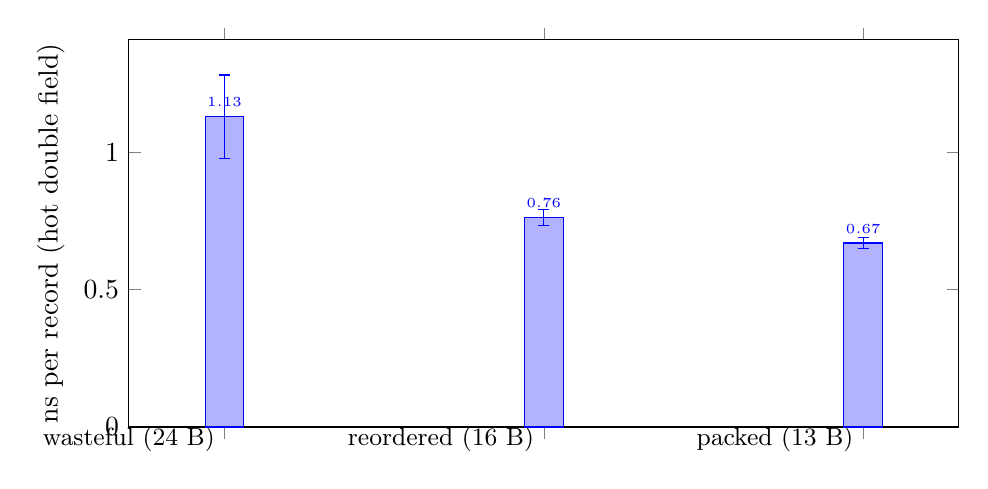
\begin{tikzpicture}
\begin{axis}[ybar, width=\textwidth, height=6.5cm, bar width=14pt, ymin=0, symbolic x coords={wasteful (24 B),reordered (16 B),packed (13 B)}, xtick=data, x tick label style={rotate=0, anchor=east, font=\small}, ylabel={ns per record (hot double field)}, enlarge x limits=0.15, legend style={font=\small, at={(0.98,0.98)}, anchor=north east}, nodes near coords, nodes near coords style={font=\tiny}, every node near coord/.append style={/pgf/number format/.cd, fixed, precision=2}]
\addplot+[error bars/.cd, y dir=both, y explicit] coordinates {(wasteful (24 B),1.1300) +- (0,0.1517) (reordered (16 B),0.7629) +- (0,0.0285) (packed (13 B),0.6701) +- (0,0.0204)};
\end{axis}
\end{tikzpicture}